\graphicspath{{chapters/images/03/}}

\chapter{Third week}

\section{General strategy to analyze a dataset}

\section{Principal Component Analysis}
Data from a big table, Starting point is a $ p x n $ matrix with \textit{p} is equal ot the number of genes and \textit{n} to the number of samples. The number of samples has to be between 40 to 100, if smaller than 20 analysis become difficult. If bigger, it is possible to use a subset of the dataset. p is normally larger than n, as of course genes are more. Source of errors are introduced, making noise. Generally a lot of non informative data, or even wrong, most often it is necessary to transform the data and normalize it. 

Formulate a question and try to answer to that, about the aim, which genes are differentially expressed between different groups. Is it possible to group samples with similar expression profile?. Think about the statistical test then. Once done the question, open data file, data normalization, transformation and PCA. Questions through the description of the experiment. 

For \textbf{class comparison}, it is possible to use a \textbf{t-test}, what are the genes whose expression is different between different groups. Statisticall significance has to be detected. T-test to understand if $H_0$ is true or the alternative hypothesys is True. The test gives a \textit{p}-value.
Calculate the $T_{observed}$. Difference obtained by chance or not? Are the data extracted from the same distribution (in this case mean of the two groups should be similar)? 
A solution is to use a correction method, like Bonferroni. The problem of \textbf{threshold} is not already solved, normally $0.05\%$. The percentage remains arbitrary. $0.05$ means that you have a mistake as result only for the 5\% of the times. 
The ones with smaller \textit{p}-value are the most interesting. It is possible to sort the genes and take those with lower values of \textit{p}-value.

Estimates of mean and standard deviation, very different values in different experiments. Especially if number of samples is low. Larger number of samples make the estimates more robust.

The \textbf{multiplicity problem} has to be considered.
For a given gene and a given type I error rate ($ \alpha=5\% $), we know that this gene has a
5\% probability to be a false positive. Thus, when doing one test at $\alpha=5\%$  for each
gene, we know that the number of false positives will be 5\% times the number of
tests (5 FP for 100 tests, 50 FP for 1000 tests,…, 2200 FP for 44000 tests).
The T-test produces more reliable results with normal distributed data.


The adjustment is made to have a new \textit{p}-value.

It is possible to \textbf{rank} the genes based on the \textit{p}-value, those with the lowest \textit{p}-value are those more interesting. take for example the first thirty, draw a heat-map, where column is a sample and row is a gene. The t-test makes assumption on data, it is not the best oprion for class comparison. You have to set a threshold, and establish which are interesting and which not. The choice of threshold is always arbitrary. 

It has to be started the analysis. Open the file, read the data, maybe to many $ 0s $. It is done a data normalization and a PCA, a way to reduce dimensionality of the dataset. 

\subsection{Normalization}
Ranges of values are presented through box-plots. The middel line is the median. Points out of whiskers are outliers. Whiskers represent 1.5 times the interquartile range %TODO .
The range of values are really disalligned, for no reason, variation in the data that has no biological explanation. Reallign the boxes through normalization.

The variation can be sistematic, same for all the samples, or it can be random. The best way to deal with radom is to do several replicates. Random variations have a 0 mean. 

The sources of variation :

Dye bias: differences in heat and light sensitivity, efficiency of
dye incorporation
Differences in the amount of labeled cDNA hybridized to each
channel in a microarray experiment (here channel is used to
refer to a particular slide/dye combination.)
Variation across replicate slides
Variation across hybridization conditions
Variation in scanning conditions
Variation among technicians doing the lab work
etc.

The general strategy for normalization is to use
House keeping genes,
considered not to change on average across samples and
conditions. Remove residual variation of house keeping genes taking a pool of these genes.

The simplest method: subtract the median from each values of the profile $\Rightarrow$ all the samples are alligned on  $0$, through the shifting up and down of the boxes. 

Variants of normalization: batch effect: source of error is known, for example different processing (very unlikely the same results), some packages are available; microarray done in different days.

Once done the alignment to 0 of the median, boxplots with the median alligned. The amplitude of the boxes is not equal, scale normalization can be done: it can be done deviding by the standard deviation for that profile for each profile, each value. To do both the normalization processes, 

%R commands and suggests to ADD %TODO
it can be used the \textbf{scale} built in function of R.  

The t-test should be done on the final version of the data. 

\textbf{\textit{MAD}} stands for "\textit{median standard deviation}". The possible presence of outliers justify the use of the median, off range, so extreme that can be produced by errors. Remove or mantain? it influences enormously the calculus of the mean and of the standard deviation. Median is not affected instead by outliers.

Other more sufisticated methods are available to normalize the data. 

\subsection{Data transformation}
There has to be a reason for that.
Replace the numerical values with $ \log $ of the values. This changes the shape distribution of the data, maybe obtaining data more normally distributed. Ranks are also usable, where each value is substitued with its position after that it is sorted from the lowest to the highest.
Z-scores are obtained after standardization of values.

The $ log $-transformation is made on graphs not normally distributed. T-test can be used on normal distributions, and this is considered as True when performing the test.

\subsection{Principal component analysis (PCA}

Also known as latent vectors, latent variates, principal axes, 
principal factors, reduce dimensionality. \textbf{Reduce dimensionality}, each sample 30000 values collection, dataset can be seen as a series of points with 30000 dimensions. Obviously, the number of dimensions has to be reduced. PCA plots are generally 2-dimensionals or 3-dimensional.

Given a sample of
n observations on a vector of p variables, with p variables/dimensions equal to 30000

\begin{equation}
{x_1, x_2, \dots, x_n} \in  \Re^p
\end{equation}

it is possible to go from a space of p dimensions to a space of n dimensions. transformation from the space of the xs to the ys. 

Using the linear regression, we are going to obtain \textit{n} coordinates transformed (transformation), where \textit{n} is equal to the number of samples. We choose the best dimension which describes the most part of the variability of our data ($ y_1 $). The second dimension has to be ortoghonal to the first one ($ y_2 $). Once we have identified those directions, the point will have new coordinates. 

eigenvectors are arrays of n values, eigenvalue.
we obtain the directions that we like, how much the stress also. Only 2 or 3 are representative of the variability of the data 

each x represent a gene, ys are said metagenes, imaginary genes, whose level of expression is given by the linear combination of all the genes. 

\begin{equation}
y_{i,j} = a_{j,1}x_{i,1} + a_{j,2}x_{i,2} + \dots + a_{j,p}x_{i,p}
\end{equation}

A few metagenes are needed to describe variability of data. Which metagenes to use? Usully the first, the second and the third are used. 

In the process $ S = B^T B $ it is the covariance matrix. If the data was standardized, correlation and covariance are the same. Correlation matrix vs covariance matrix %TODO .

\textbf{in R...}: \textit{prcomp} is built-in into R. Array of colours to be used. one gene per row and a sample per column, in some cases, as for \textit{prcomp}, it is needed the inverse arrangement. 

In new set of coordinates, directions should be orthogonal, the first ax should be the one over which the cloud of points is more stratched. 

If data is a ball, data obtained by random. The way to obtain the coefficients so that it is satisfied ... is to use the covariance matrix, obtained through the multiplication of the matrix per itself transposed. Take the eigenvectors, each one is a row of that matrix, while instead the eigenvalues provide an estimate of the percentage of the variability of the corresponding axes is out of the total variance (how spread along that direction).

The covariance matrix is symmetric and positive. As a consequence, all the eigenvalues are positive. 

computations of eigenvalues and eigenvectors are made through a function. Coordinates of the points in the new set of coordinates as output. 

The skree diagram make us see which components are relevant

Scores %TODO


\begin{figure}[h]
\caption{Scree diagram}
\centering
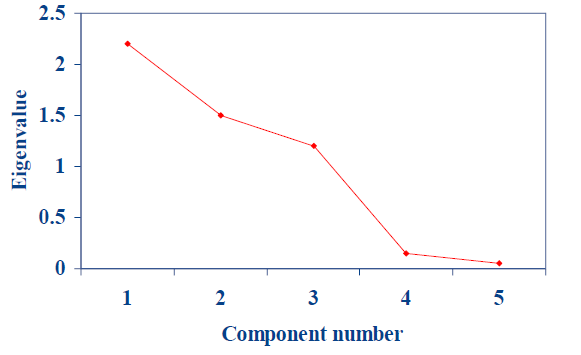
\includegraphics[width=0.6\textwidth]{skreeDiagram}
\end{figure}


\begin{itemize}
	\item \textbf{Inspect dataset:} check data in there, not too many NAs. 
	\item \textbf{Normalization}: The sistematic source of variation can be eliminated by using a box-plot, which means great amount of variation. normalization is made by subtracting the median.
Align the size of the boxed by aligning the standard deviation
	\item \textbf{PCA}:
\end{itemize}



\subsection{Series Matrix of GEO}
on the left column, there are present informations regarding the authors, date, platform (GEO assigns it), the type. Each line starts with !, which indicates this is a piece of metadat. The second section is specific to each sample. The third section contains the data. 



